% Chapter Template

\chapter{Haskell Type Checking} % Main chapter title

\label{chap:haskell-type-checking}

\graphicspath{{Figures/HaskellTypeChecking}}

In this chapter we delve into the more technical aspects of type checking Haskell programs. We first define a small subset of the Haskell language, and take a look at the typing rules that govern what constitutes a well typed program and what not using the Hindey-Milner type system. In the second half we explore the notion of constraint based type checking, and how it compares to the Hindley-Milner based type checking.

\section{The language and syntax}
We start our discussion by defining a subset of the Haskell language. This language H is  an expression based functional language, which includes features like type annotation, polymorphic types, let expressions and a few ground types. The syntax of the language is shown below. The formal semantics of this language is  out of our concerns, because our scope is the type-checking phase which occurs before the program being executed.


\begin{figure}[hbt]
    \includegraphics[width=\linewidth]{LanguageSyntax}
    \caption{
      The syntax of a small functional language that we will be using to discuss the type-checking approaches
      }
  \end{figure}


The real world Haskell includes more features. However, this is done by a series of transformations whereby the semantics of the core language is quite minimal.


\section{Haskell Type Inference and Algorithm W}

The Hindley-Milner Type System (HM) and Algorithm W are foundational parts of type inference in many functional programming languages, including ML, Haskell, and Elm. The Hindley-Milner Type System, named after its inventors Roger Hindley and Robin Milner, is a type system that can automatically infer the types of expressions in a language with no annotations required. The system provides polymorphic typing, meaning that a variable can be assigned multiple different types automatically based on its usage context, making it easier to write flexible, reusable code without compromising type safety.

\begin{figure}[hbt]
    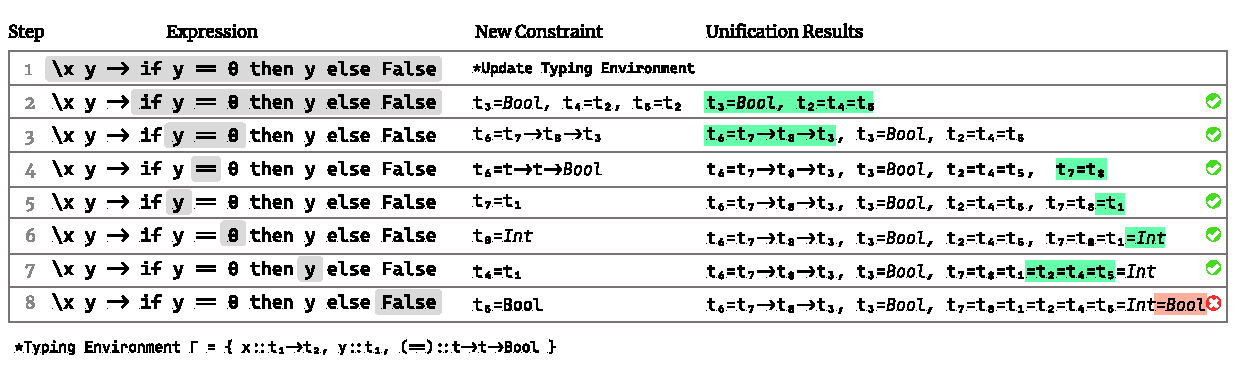
\includegraphics[width=0.5\linewidth]{HindleyMilner}
    \caption{
        The declarative typing rules of the Hindley-Milner type system.}
\end{figure}



\textbf{Algorithm W} is the algorithm that performs type inference in the Hindley-Milner type system. It was initially designed for the ML language. The purpose of this algorithm is to achieve efficient and correct type inference.


Algorithm W works by first assuming that each expression has a unique type variable associated with it, and then linking these variables together in equations using the language's typing rules. Finally, it solves these equations using unification, a process that finds a substitution which makes both sides of an equation equal. Throughout this process, Algorithm W also performs "let-polymorphism," whereby a variable bound by a "let" statement can take different types in different contexts.


\textbf{Algorithm M} is a variant of Algorithm W, but it's designed to be more efficient. It aims to reduce the amount of type information that needs to be maintained, and to minimize the amount of type reconciliation required. Algorithm M, like W, is meant to handle polymorphic type inference, but its major difference lies in the way it handles let-polymorphism, making it more suitable for modern functional programming languages as it is more modular.


Together, the Hindley-Milner type system and Algorithm W/M form one of the most important foundations for functional programming languages. They allow for flexible, clear, and correct code, and all without explicit type annotation.

\section{Constraint-based Type Inference}

Constraints programming is a programming paradigm where programmers describe the constraint of a feasible system based on the decision variables. Constraint programming has been widely used in optimization and artificial intelligence. In the context of type checking in programming languages, constraint programming can prove useful. In this case, each expression is associated with a type variable that represents the type it will eventually hold. The task of type solving becomes finding an instantiation for the constraint program.

\subsection{Notable Constraint/Logic Systems to Model Types}

\subsubsection{Satisfiability modulo theories}


\begin{figure}[hbt]
  \includegraphics[width=\linewidth]{MaxSMT}
  \caption{An Type Relation Encoding based on MaxSMT}
\end{figure}

Satisfiability modulo theories (SMT) is a flexible language that extends SAT by allowing variables to have domain-specific types and relationships. Many studies focus on encoding typing relations as SMT programs. This approach can be benefited from many mature SMT solvers that perform efficient searches. These solvers include Z3 (by Microsoft Research), CVC4, and Yices.

\subsubsection{Constraint Handling Rules}
Constraint Handling Rules (CHR) is a high-level programming language based on multi-headed, forward chaining (or left-to-right) rules. Originally developed for writing user-defined constraint solvers, CHR is now recognized as a general-purpose language, due to its concurrent and rule-based nature. Chameleon uses CHR to model the type system of Haskell types.

\subsection{Prolog}
Prolog is a logic programming language. Although not a constraint language by definition, prolog itself can be used as a constraint language by ignoring its logic programming constructs. The main difference is that prolog provides a convenient system for creating user-defined predicates, where constraint languages focus on expressing constraints. However, to a certain extent, the standard prolog is capable of expression constraints posed by a typical type system. On top of that, most prolog distributions provide constraint logic modules such as cpl in SWI prolog.


We provide an encoding of Haskell typing in prolog language. In this encoding. [More details of the encoding]


\begin{figure}[hbt]
  \includegraphics[width=\linewidth]{Prolog}
  \caption{An Type inference defined in prolog predictes}
\end{figure}
  
\section{The analysis of an unsatisfiable system}

One advantage of using a constraint based type system is that it offers many tools to understand the unsatisfiability of a system. In terms of programming language, the most useful tool we use is Minimal Unsatisfiable Subset (MUS).  MUS detection aims to find the smallest subset of constraints that still renders the system infeasible. For an ill-typed program, this means finding a minimal set of locations that contain a type error. Although finding such a subset can be computationally expensive, it is useful because it represents the type error in more than one location, and contains two sides of the conflict. This is often necessary knowledge in understanding any kinds of conflicts.


Other than MUS, minimal correction set (MCS) and  maximal satisfiable subset (MSS) are useful subsets of the constraint system as well. We give the formal definition of these subsets and their type theoretic interpretation.


[More examples from the prev section]


– A minimal unsatisfiable subset (MUS) $M$ of a constraint system $C$ is a subset $M \subseteq C$ such that $M$ is unsatisfiable and $ \forall{c} \in M : M \setminus \{c\}$ is satisfiable. An MUS can be seen as a minimal explanation of the infeasibility of the constraint system. MUSes have been used extensively, mostly in combination with programming slicing, as a means to explain type errors. An MUS of type system constraints encode a path of reasoning connecting all evidence from one location of the conflict to another.


– A minimal correction set (MCS) $M$ of a constraint system $C$ is a subset $M \subseteq C$ such that $C \setminus M$ is satisfiable and $\forall{S} \subset M : C \setminus S$ is unsatisfiable. MCSes are so named because their removal from $C$ can be seen to “correct” the infeasibility. In an ill-typed program, an MCS can be seen as the ``cause" of a type error; removing any MCS will result in the system being well-typed. Goanna uses an MCS to represent potential causes of a type error. Each MCS contains the set of locations that need to be changed to fully resolve the type error.

  

– A maximal satisfiable subset (MSS) $M$ of a constraint system $C$ is a subset $M \subseteq C$ such that M is satisfiable and $\forall{c}\ in\ C \setminus M:M\cup\{c\}$ is unsatisfiable. The definition of an MSS is symmetric to that of a MUS, with `satisfiable' and `unsatisfiable' swapped along with maximal for minimal. MCS and MSS are complement sets of each other. In an ill-typed program, an MSS can be seen as the resulting typing environment if a type error is fixed by relaxing the MCS.

\subsection{MUS Enumeration}
One observation we can make about the  Minimal Unsatisfiable Subsets is that it is often not unique . It is possible for an unfeasible system to contain a finite number of MUS’s. In practice, existence of multiple MUSs indicates that there are multiple sources of conflict. Enumerating multiple MUS/MCS in this case may provide better insights over the root cause and how to address them properly


However, the problem of MUS enumeration is that it is very computationally expensive. In the most naive approach, it requires exploring the powerset of all constraints in the constraint system. In fact, most of the effective enumeration algorithms today rely on heuristics, and they provide performance improvements on a case-by-case basis. MARCO~\cite{} and MUST~\cite{} are examples of such an approach. They use heuristics to avoid traversing a large chunk of the subsets each representing a permutation of which constraints to be relaxed and which not.


\begin{figure}[hbt]
  \includegraphics[width=\linewidth]{MarcoAlgo}
  \caption{An simple implementation of the MARCO algorithm}
\end{figure}


\begin{figure}[hbt]
  \includegraphics[width=\linewidth]{MarcoViz}
  \caption{An illustration of how MARCO finds all MUSes}
\end{figure}
  

\section{Three Classes of Type Error}

I propose an useful categorization of type errors. This categorization allow a formal study of the tools that is necessary to cover the information of a given type error.  Because we have covered MUS and MUS enumeration, it is now possible to discuss 3 categories of type error based on the feasibility of representing them in a single MUS.

\subsection{Multi-step Type Error}
\begin{figure}[hbt]
  \includegraphics[width=0.5\linewidth]{Multi-step}
  \caption{}
\end{figure}

Multiple-step type errors contain a chain of reasoning steps, or a series of attempts to unify two logical terms. There is no possible way to successfully complete all the unifications. However, removing any one of the unification steps will make all other steps feasible. In the error presented in the above figure, the error can be represented in a single MUS {A, B, C, D}.

\subsection{Multi-witness Type Error}
\begin{figure}[hbt]
  \includegraphics[width=0.5\linewidth]{Multi-witness}
  \caption{}
\end{figure}
A Multiple-witness type error occurs when one side of the conflict contains multiple locations (witnesses) suggesting the same typing assignment. Removing one such location, the type error will remain. In the example, there are three MUSes: {A, D}, {B, D}, {C, D}. Therefore, this type of error cannot be succinctly represented by a single MUS.

\subsection{Multi-party Type Error}
\begin{figure}[hbt]
  \includegraphics[width=0.5\linewidth]{Multi-party}
  \caption{}
\end{figure}

A Multiple-party type error is an error where multiple type irreconcilable assignments can be obtained from locations of the source code. In the provided example, there are 3 MUS: {A, B}, {A,C}, {B,C}. Therefore, this type of error cannot be succinctly represented by a single MUS.

\begin{figure}[hbt]
  \includegraphics[width=\linewidth]{Compare}
  \caption{}
\end{figure}

\section{Conclusion}
In this chapter, we established a subset of the Haskell language by defining its syntax, and typing rules. We explored two avenues to type-check a program in such language and obtain principle types: using the Hindley-Milner type system and using constraint-based type system. In addition, we explored some type error analysis tools that are enabled by using a constraint based type system, and how these tools are applied to three different kinds of type errors. We will explore them in the next two chapters.